\documentclass[12pt,francais]{report}

\usepackage[UTF8]{inputenc}
\usepackage[pdftex]{graphicx}
\usepackage[french]{babel}
\usepackage{enumitem}
\usepackage{scrextend}
\usepackage{float} 

\begin{document}

\begin{center}

\includegraphics[scale=0.3]{./images/logo_universite_orleans.png}~\\[1.5cm]

\textsc{\large Master 1 - TER}\\[1cm]	

\rule{\linewidth}{0.5mm}\\[0.4cm]

{ \LARGE \bfseries GoodLua\\[0.4cm] }

\rule{\linewidth}{0.5mm}\\[2cm]
\end{center}


\begin{minipage}{0.4\textwidth}
      \begin{flushleft}
			\textsc{Bovie} Pierre-Edouard\\
			\textsc{Labourbe} Loïc\\
			\textsc{Maslowski} Antoine\\
			\textsc{Roche} Julie\\
			\end{flushleft}
    \end{minipage}\hfill
    \begin{minipage}{0.6\textwidth}
      \begin{flushright}
			Enseignants : \textsc{Couvreur} Jean-Michel\\
			\textsc{Dabrowski} Frederic\\

\end{flushright}
    \end{minipage}\\[1.5cm]
		
		\begin{center}
    {7 Février 2018 - 25 Mai 2018}
		\end{center}
	
\chapter*{Partie documentaire}	

\section*{Résumé du projet}	

L’objet du projet est la conception d'un système pour la création et le lancement à distance de programme Lua s'exécutant sur un robot. Le système matériel est composé d'une tablette Androïd et d'un robot mobile à base pcDuino équipé de divers capteurs. Le logiciel de la tablette offrira la possibilité : 
\begin{itemize}
\item de concevoir des programmes
\item de charger à distance le programme sur le robot 
\item de télécommander le robot 
\end{itemize} 
Le système logiciel sur le robot permettra de recevoir et d'exécuter les programmes Lua transmis par la tablette.
		
\newpage 
\section*{Introduction au domaine}

\paragraph*{Quelles sont les possibilités de Blockly ?\\}

Blockly a principalement deux utilités. La première est l'apprentissage de la programmation via un moyen visuel, et la seconde est le développement de programmes embarqués, notamment en robotique.
	
La simplicité d'utilisation de Blockly en fait un outil d'apprentissage très pratique, et ce dès le plus jeune âge. En effet, il suffit de choisir puis glisser des blocs, afin de les imbriquer, comme des pièces de puzzle. Plusieurs sites, jeux et applications proposent des moyens ludiques basés sur Blockly pour apprendre à programmer. Le site le plus connu est celui proposant la série des 'Blockly Games' \cite{ref12}. Existant dans un très grand nombre de langues, il contient plusieurs jeux, de 10 niveaux chacun, avec une augmentation progressive de la difficulté de niveau en niveau et de jeu en jeu afin de découvrir le développement. Le premier de ces jeux est un simple puzzle sur les animaux, afin de découvrir le fonctionnement de Blockly. Le second jeu est un labyrinthe qui utilise des conditionnelles et des boucles. Le jeu suivant, qui permet de diriger les déplacements d'un oiseau, rentre plus sérieusement dans les 2 thèmes du jeu précédent. Suit un jeu qui fait découvrir le dessin via la programmation, puis un autre qui permet de créer des animations évoluant selon le temps. Enfin, on est amené à coder un petit jeu de tir, tout d'abord avec des blocs, puis en JavaScript à partir de ces blocs. Il existe plusieurs autres séries de jeux basés sur Blockly, on peut notament citer 'Rapid Router' \cite{ref13} qui en 100 niveaux initie les enfants au Python. Ces jeux, généralement accessibles à partir de 8 ans, sont une solution ludique, permise par Blockly pour initier les plus jeunes à la programmation.

Blockly est également utilisé en robotique, dans de nombreux projets. En effet, la bibliothèque étant libre, elle permet de coder ses propres blocs. Les utilisateurs de robots peuvent donc pré-coder les différentes fonctionnalités, et n'ont donc plus qu'à les assembler dans la séquence souhaitée lors de l'exécution. Encore une fois, cette manière d'utiliser Blockly, bien que pratique pour faire du développement embarqué, est aussi et surtout un moyen d'apprendre simplement la programmation sur robot. Par exemple, le robot 'Thymio' \cite{ref14} est un petit robot qui permet de découvrir l'univers de la robotique et sa programmation. Ce robot fournit une intégration de Blockly, qui permet \textit{"de le programmer de façon purement événementielle"}. Un environnement 'Blockly4Thymio' \cite{ref15} a également été ajouté au projet, et offre un apprentissage ludique, destiné à un jeune public.

A l'exception de quelques jeux, généralement mobiles, destinés au grand public et basés sur la librairie Blockly, sa principale utilisation reste donc dans un but éducatif, comme l'avait prévu Google en la créant.


\paragraph*{Quels sont les autres moyens visuels d'apprentissage de la programmation ?\\}

De nos jours de nombreux langages sont développés dans le but de pouvoir enseigner à programmer. Ces langages ont tous des particularités qui permettent de faciliter l'utilisation par des personnes qui sont peu familières avec le monde du développement et peuvent être classés selon deux grandes catégories.

La première regroupe des langages disposant de syntaxes simples ce qui permet une utilisation simple due au fait que l'on traduit d'une manière naturelle ce que l'on attend de notre programme en un code. De plus ces langages sont également utilisés pour développer de réels projets, ce qui permet d'apprendre avec un langage simple mais qui peut être utilisé dans le domaine professionnel. Des exemples pour ces types de langage sont : Python, Ruby.

Le deuxième groupe rassemble des langages visant plus à apprendre le concept de comment programmer plutôt que de réellement apprendre un langage de développement. Pour cela il se base sur une interface graphique simple d'utilisation, le plus généralement les fonctions, actions et événements ont la forme de bloc  que l'utilisateur combinent les un avec les autres en les faisant glisser. Cette catégorie comprend des langages telle que 'Scratch' \cite{ref17}, qui est actuellement utilisé dans les écoles et collèges, 'Alice' \cite{ref19} et 'LEGO Mindstorm Robotics' \cite{ref18}. Ce dernier est d'ailleurs utilisé dans le but d'enseigner le développement pour la robotique car il  permet de programmer des robot tout en restant simple d'utilisation.

\textit{"Most jobs in the future will most likely have some sort of connection to coding"}  Navdeep Bains, Ministre canadien de l'innovation,des science et du dévelopement econimique.

\textit{“ICT used to focus purely on computer literacy – teaching pupils, over and over again, how to word-process, how to work a spreadsheet, how to use programs already creaking into obsolescence; about as much use as teaching children to send a telex or travel in a zeppelin.
Our new curriculum teaches children computer science, information technology and digital literacy: teaching them how to code,and how to create their own programs; not just how to work a computer, but how a computer works and how to make it work for you.”}
Michael Goove, secrétaire d'état a l'éducation du Royaume-Uni (2010-2014) \cite{ref16}

\paragraph*{Comment apprendre à développer grâce à des robots ?\\}

Des personnes ou des sociétés de plusieurs horizons ont cherché à rendre accessible l'apprentissage de la programmation via des robots, en voici quelques exemples :

Jacqueline M. Kory Westlund est une chercheuse travaillant au MIT. Son domaine de recherche est les interactions entre l'homme et la machine.
Elle crée des robots pour les enfants et étudie leurs relations et les possibilités d'apprentissage.\cite{ref9}
Le robot est dirigé par une application sous Android.

'Cozmo' est un robot développé par la société Anki. Ce robot possède la technologie 'Code Lab', qui est basée sur Scratch.\cite{ref10} 
'Code Lab' possède une interface graphique intuitive et propose une manière simple de programmer le robot.
Chaque fonctionnalité est représentée par un bloc d'une certaine forme.
Ces blocs s'assemblent les uns dans les autres et permettent à un utilisateur sans connaissance en programmation d'ajouter une nouvelle fonctionnalité au robot.

'Hexa' est un robot produit par la société Vincross. Devant l'absence d'OS orienté robot, ils ont créé le leur: 'MIND' \cite{ref11},
basé sur une architecture Linux. De nombreuses librairies sont proposées afin de contrôler facilement le robot.
Une de leurs librairies propose une interface 3D afin de permettre aux non-développeurs de créer des mouvements et des comportements complexes.
Une application est disponible sur iOS et android pour contrôler le robot à distance.

\paragraph*{Quelles sont les possibilités de l'embarqué ?\\}

La programmation embarquée est un vaste domaine, allant des systèmes embarqués de voitures à tous les objets connectés de la maison, et est décomposable en de nombreux sous-domaines. Nous allons ici plus particulièrement nous intéresser aux possibilités offertes par l'arduino en matière d'embarqué.

La domotique est l'un des champs d'utilisation d'un arduino \cite{ref20}. Grâce à leur petite taille, beaucoup d'objets domestiques sont contrôlés par des arduinos. Prenons par exemples quelques objets que l'on peut utiliser dans son jardin, et qu'il est possible de créer soi-même, ou qui existent dans le commerce, et qui utilisent un arduino \cite{ref21}: 

- un verrou électrique à code, pour sécuriser un portail, contrôlé par un arduino, et composé d'un verrou, d'un clavier et d'un afficheur LED, auquel on peut aussi ajouter un lecteur de badges RDID (identification par radiofréquence).

- un arrosage automatique, composé d'une sonde de détection d'humidité, une vanne électromagnétique, et une carte arduino, qui selon le niveau d'humidité du sol va activer un arrosage.

- un lampadaire, qui grâce à un capteur de lumière et un arduino pourra s'allumer de la tombée de la nuit jusqu'à une certaine heure.

- une station météo, qui pourra surveiller la luminosité, la température et l'humidité, et vous prévenir sur votre smartphone.

Arduino est également beaucoup utilisé en robotique, car ces cartes permettent de contrôler plusieurs éléments, d'autant plus lorsqu'elles sont associées à un micro-ordinateur (Raspberry Pi, pcDuino). Par exemple, une carte pourra contrôler l'activation des moteurs, tout en surveillant leur chaleur grâce à un capteur, et les arrêter en cas de surchauffe. Elle pourra aussi recevoir des informations transmises par des capteurs infrarouges, ultrasons, ou même une caméra, et réagir en conséquence. \cite{ref22}

Les champs des utilisations d'arduino étant très vaste, l'imagination de sa communauté d'utilisateurs en est la seule limite. Parmis les projets sortant de l'ordinaire, ont été créés un fauteuil roulant motorisé avec joystick \cite{ref23}, des jouets tels que des petits trains autonomes ou des voitures télécommandées, un gps, des volets roulants connectés, un incubateur d'oeufs connecté \cite{ref24}, et bien d'autres.


\newpage
\section*{Analyse de l'existant}

Nous avons reçu pour ce projet, un kit matériel qui forme le robot.\\
Pour nous aider à découvrir son utilisation, nous avons étudié le projet d'algorithmique répartie des étudiants de la promotion 2015 des master 1 informatique \cite{ref1} dans lequel ils manipulent un robot semblable au notre, mais avec des des langages différent du notre (Lua) puisqu'ils l'ont contrôlé avec du python et du C++.

\begin{figure}[!h]
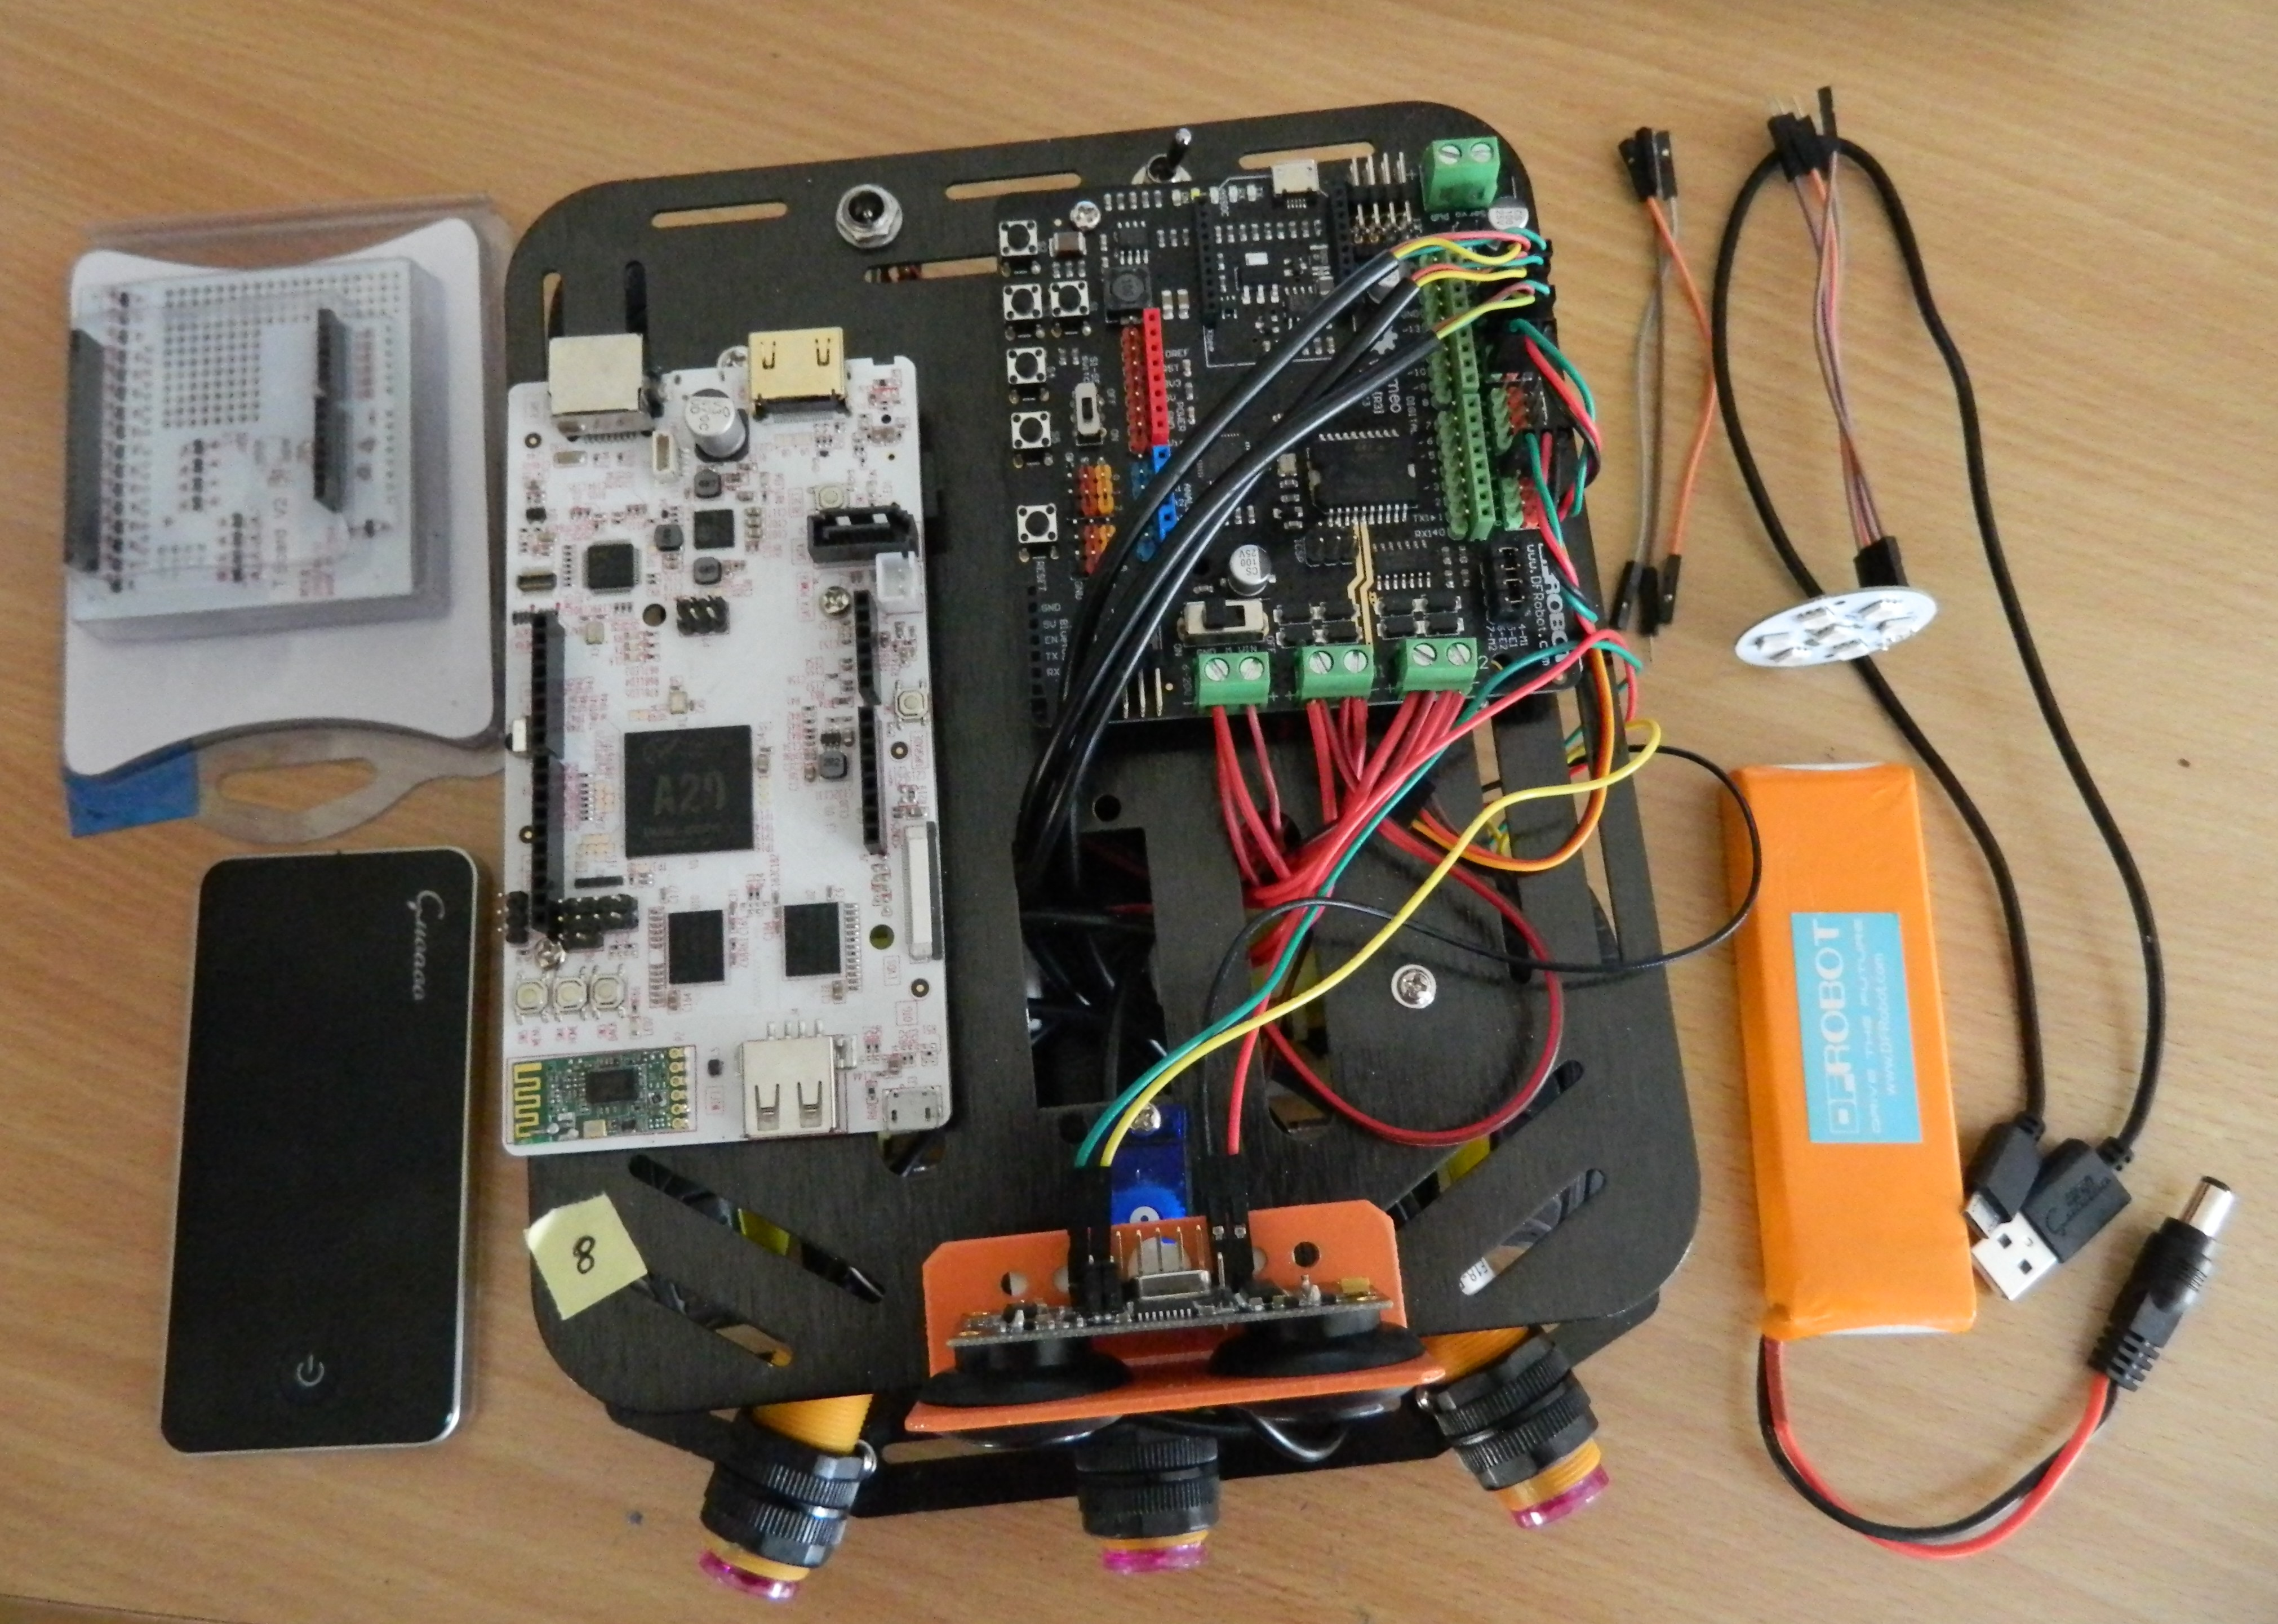
\includegraphics[scale=0.4]{./images/notre_materiel.jpg}~\
\caption{Notre materiel}
\end{figure}
	
Voici la liste du matériel dont nous disposons et dont nous devrons nous servir pour ce projet :

\begin{description}
\item [Le pcDuino :] La carte pcDuino V3 est un mini PC possédant un processeur dual core A20. Une fois branchée à un écran, un clavier et une souris, grâce à son port USB, elle s'utilise de la même manière qu'un PC sous une distribution Ubuntu. Elle possède un lecteur de carte micro-sd,  c'est dans cette carte que se situe le système d'exploitation du pcDuino. Le pcDuino possède également un port ethernet ainsi qu'une carte wifi, ce qui permet de se connecter à un réseau facilement. Pour le faire fonctionner, il suffit de le brancher à un chargeur USB par son port micro USB. Il possède enfin des broches arduino, en plus de ses interfaces de communication, permettant de faire de la programmation arduino.\cite{ref3}
\item [L'arduino :] L'arduino Romeo V2.2 (R3) \cite{ref4} est un micro-contrôleur tout en un spécialement créé pour la robotique, qui fournit des interfaces de puissance pour contrôler des moteurs.
\item [La plateforme mobile :] Notre robot est composé d'une châssis Baron - 4WD auquel sont associés 4 moteurs reliés à 4 roues codeuses. \cite{ref5}
\item [La LED :] Le disque contient 7 LEDs RGB \cite{ref6}, que l'ont peut allumer grâce à 3 pins, un pour chaque couleur, ainsi qu'avec un pin d'alimentation.
\item [Les capteurs infrarouges :] Les 3 capteurs possèdent une LED qui s'allume si un objet est dans le champ de détection. Ils ont une sortie binaire, selon si un obstacle est détecté ou non. Leur distance de détection peut être de 3 à 80 cm, et se règle manuellement avant l'utilisation. \cite{ref7}
\item [Le capteur ultrasons :] Lié à l'arduino, il détecte des températures allant de -10 à environ 70 degrés celsius, à une distance de 4cm, jusqu'à 5m. \cite{ref8}
\item [La clé bluetooth :] Nous avons rajouté une clé bluetooth au robot, branché sur un hub USB, qui permettra la communication avec d'autre appareils.
\end{description}

\bigskip
\begin{description}
\item [Blockly :] Nous utilisons la bibliothèque Blockly \cite{ref2} pour avoir un éditeur de code visuel. Blockly se présente sous forme de pièces de puzzle, chacune représentant un concept de code, comme une fonction, une condition, une boucle ou une variable. L'utilisateur n'a donc qu'à sélectionner et faire glisser les pièces pour les placer et les  imbriquer, afin de former un programme. Il n'a donc pas à s'occuper de la syntaxe, puisque les formes des pièces lui indiquent où il peut les placer ou non. Une fois le programme formé, Blockly peut le transformer en différents langages (JavaScript, Python, PHP, Dart) dont celui qui nous intéresse pour ce projet, le Lua.\\
Grâce à cette bibliothèque, nous avons la possibilité de créer les blocs de notre choix, correspondant à des fonctions à appliquer sur le robot, d'intégrer l'éditeur Blockly à notre application Androïd, et de générer le code à exécuter.
\end{description}

\chapter*{Cahier des charges}

\section*{Besoins fonctionnels}

\begin{itemize}[label=\textbullet]
	\item \textbf{Exécuter du code}
	\begin{description}
		\item \textit{description :} exécuter du code eLua sur le PcDuino
		\item \textit{priorité :} très haute
		\item \textit{justification :} cette fonctionnalité est la principale. Nous devons être en mesure de faire fonctionner le robot grâce à du code eLua avant toute autre chose.
		\item \textit{test prévu :} test d'exécution simple, l'équivalent du "Hello world" sur pcDuino, c'est à dire l'allumage d'une LED via du code Lua.
	\end{description}
	\item \textbf{Connecter android au robot grâce au bluetooth}
	\begin{description}
		\item \textit{description :} utiliser la clé bluetooth connectée au pcDuino pour le connecter à un appareil androïd possédant aussi le bluetooth.
		\item \textit{priorité :} haute
		\item \textit{justification :} le code crée via l'application androïd doit être transmis au robot pour être exécuté. Une solution filaire étant peu pratique, nous le connecterons via bluetooth.
	\item \textit{test prévu :} envoi de fichiers et de commandes de la tablette vers le pcDuino, et inversement.
	\end{description}
	\item \textbf{Transformer blockly en code}
	\begin{description}
		\item \textit{description :} traduire les blocs de la librairie Blockly dans le langage Lua ou Arduino.
		\item \textit{priorité :} moyenne
		\item \textit{justification :} le robot étant "guidé" par du code Lua ou Arduino, il est nécessaire de procéder à une traduction du programme visuel dans ce langage avant de l'envoyer au robot pour être exécuté.
	\end{description}
	\item \textbf{Créer un programme}
	\begin{description}
		\item \textit{description :} la création d'un nouveau programme blockly via l'application androïd.
		\item \textit{priorité :} moyenne
		\item \textit{justification :} c'est la fonctionnalité de base de l'application, il faut pouvoir créer de nouveaux programmes en vue de les écrire et de les exécuter.
	\end{description}
	\item \textbf{Sauvegarder / Charger des programmes}
	\begin{description}
		\item \textit{description :} l'utilisateur pourra sauvegarder le programme sur lesquel il travaille, et reprendre sa progression là où il était en chargeant le dernier programme.
		\item \textit{priorité :} basse
		\item \textit{justification :} cela permettra de travailler sur un programme en plusieurs fois sans risque de perdre son travail.
		\item \textit{test prévu :} enregistrer un programme blockly, fermer l'application, puis la rouvrir et charger le programme.
	\end{description}
\end{itemize}

\bigskip

\section*{Besoins non fonctionnels}

\begin{description}
	\item [Environnement de travail :]Nous travaillons sous une distribution Ubuntu. Pour la partie programmation en Lua\cite{refLua} il est possible d'utiliser n'importe quel éditeur de texte, puis de compiler le fichier. Pour la programmation en langage Arduino, nous pouvons utiliser l'Arduino IDE ou compiler et exécuter en lignes de commandes.
	\item [Rapidité d'exécution :] Il serait préférable que l'exécution d'un programme se fasse de manière assez rapide, pour ne pas aller contre les attentes de l'utilisateur. Par exemple, si le programme utilise des capteurs, mais qu'une lenteur dans le programme fait qu'un obstacle n'est pas détecté à temps, cela nuira à l'expérience de l'utilisateur. De même, l'un des buts de l'application, est de pouvoir exécuter une séquence, ou de donner des ordres au robot en temps réel. 
	\item [Simplicité d'utilisation : ]L'application doit être utilisable par des utilisateurs sachant programmer, qui pourront créer un programme complexe à partir des blocs basiques, mais elle doit également être accessible à des utilisateurs débutants en programmation, qui pourront utiliser des blocs représentant des fonctions toutes faites concernant le robot (par exemple : allumer LED). Les blocs et l'interface devront donc être instinctifs et simples d'utilisation.
	\item [Empreinte mémoire :] Le poids de l'application Androïd doit être le plus petit possible car la tablette possède une mémoire limitée.
	\item [Empreinte énergétique :] L'application ne doit pas surconsommer la batterie de la tablette, pour cela nous allons contrôler l'utilisation des ressources.
\end{description}

\section*{Prototype - l'interface de l'application Androïd }
En ouvrant l'application, l'utilisateur se verra proposer de créer un nouveau programme, il devra alors lui donner un nom. Une fois le programme créé, il aura le choix de le modifier ou de l'exécuter. [Figure 1]

Dans le cas du choix de modifier le code, on ouvrira l'éditeur visuel contenant Blockly avec l'ensemble des blocs disponibles dans une barre latérale gauche. Un menu permettra également de sauvegarder le programme en cours d'édition, de charger le dernier programme enregistré ou de l'effacer. [Figure \ref{figMaquette}]\\

\begin{figure}[!h]
\begin{addmargin}[-7em]{0em}
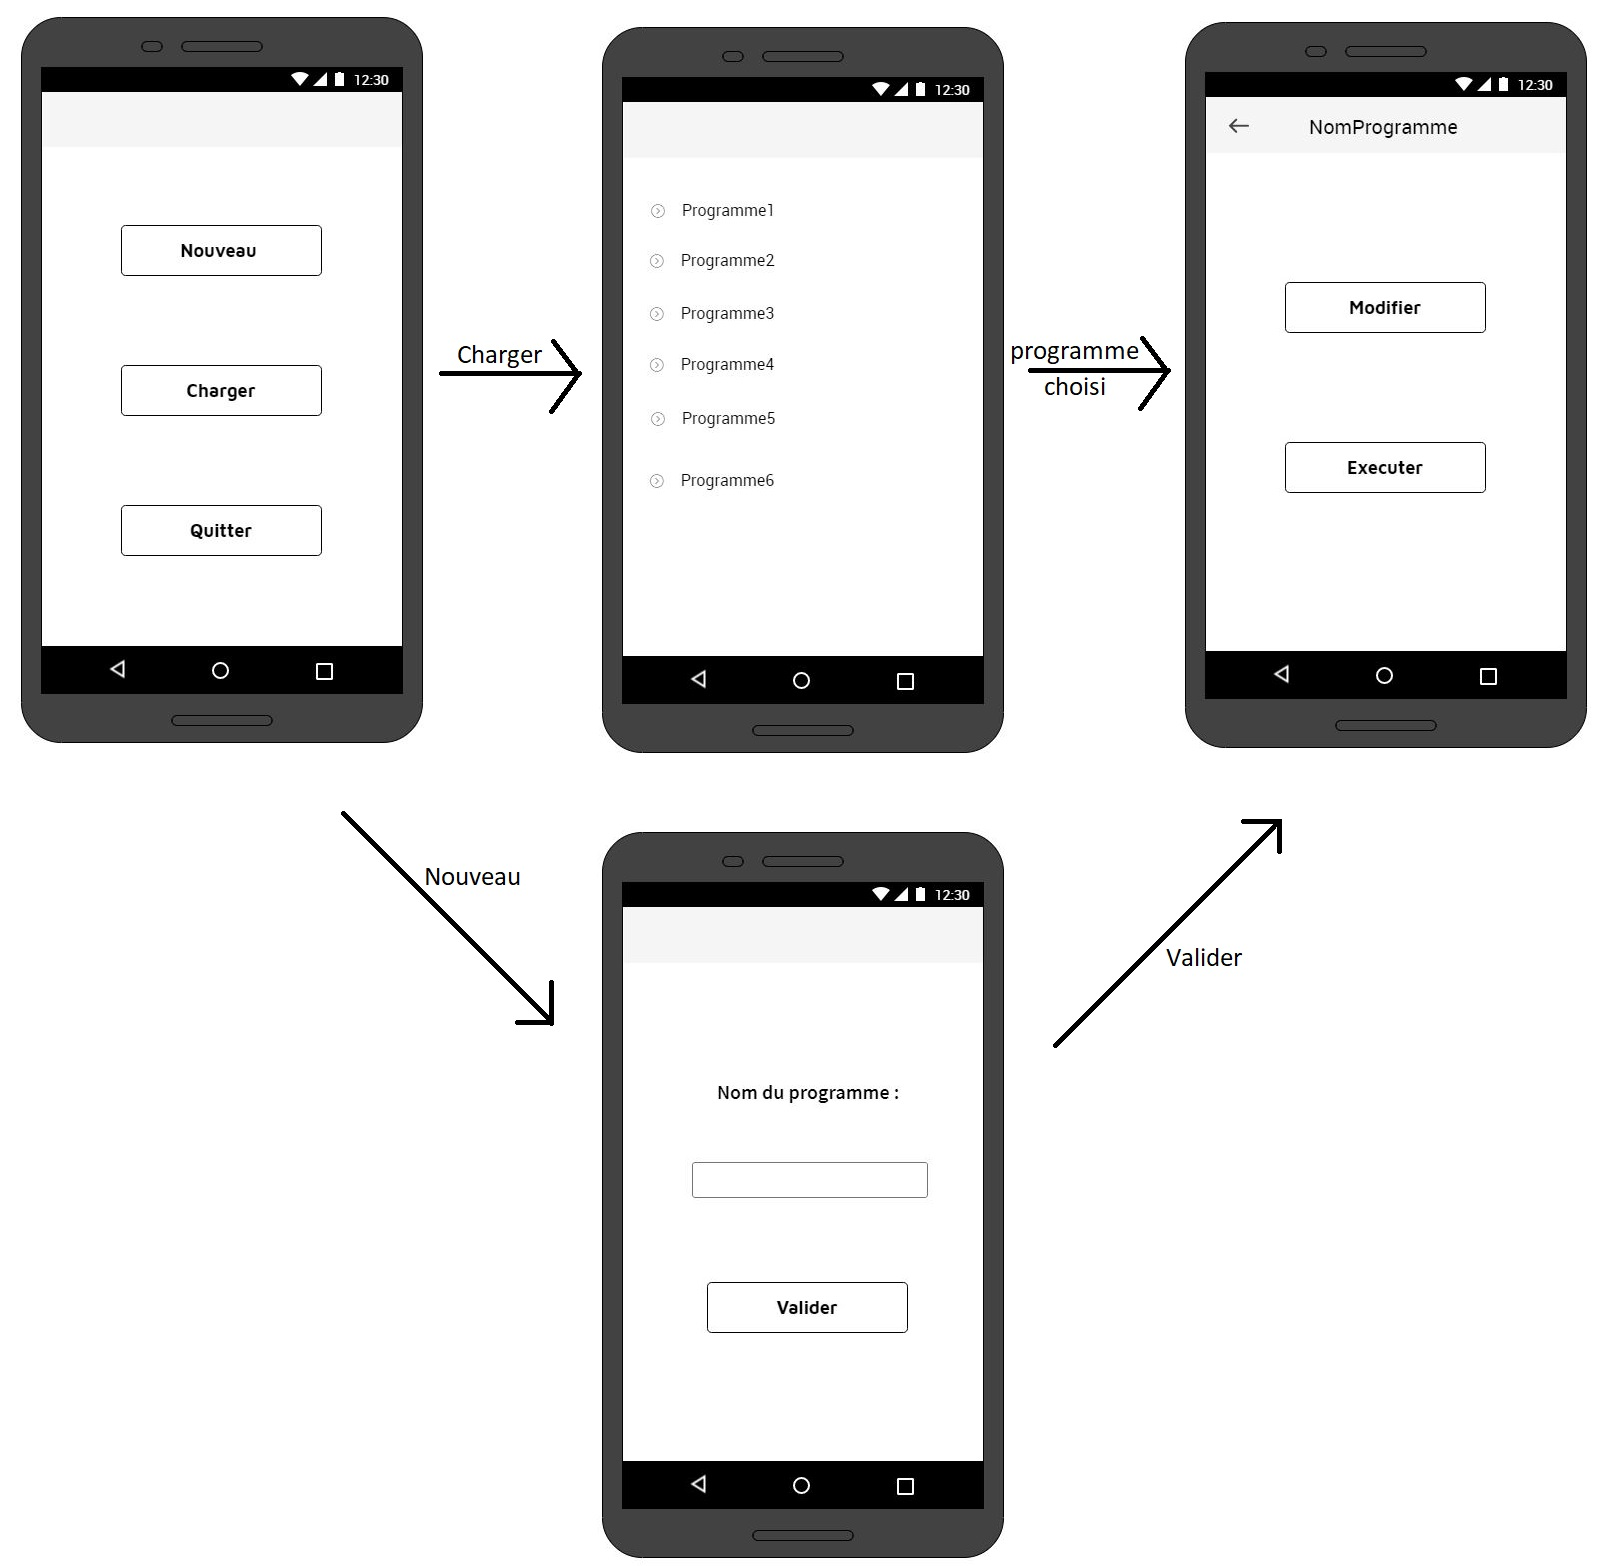
\includegraphics[scale=0.45]{./images/maquette1.jpg}~\\[1.5cm]
\caption{Maquette 1ère partie}
\end{addmargin}
\end{figure}

\begin{figure}[!h]
\begin{addmargin}[6em]{0em}
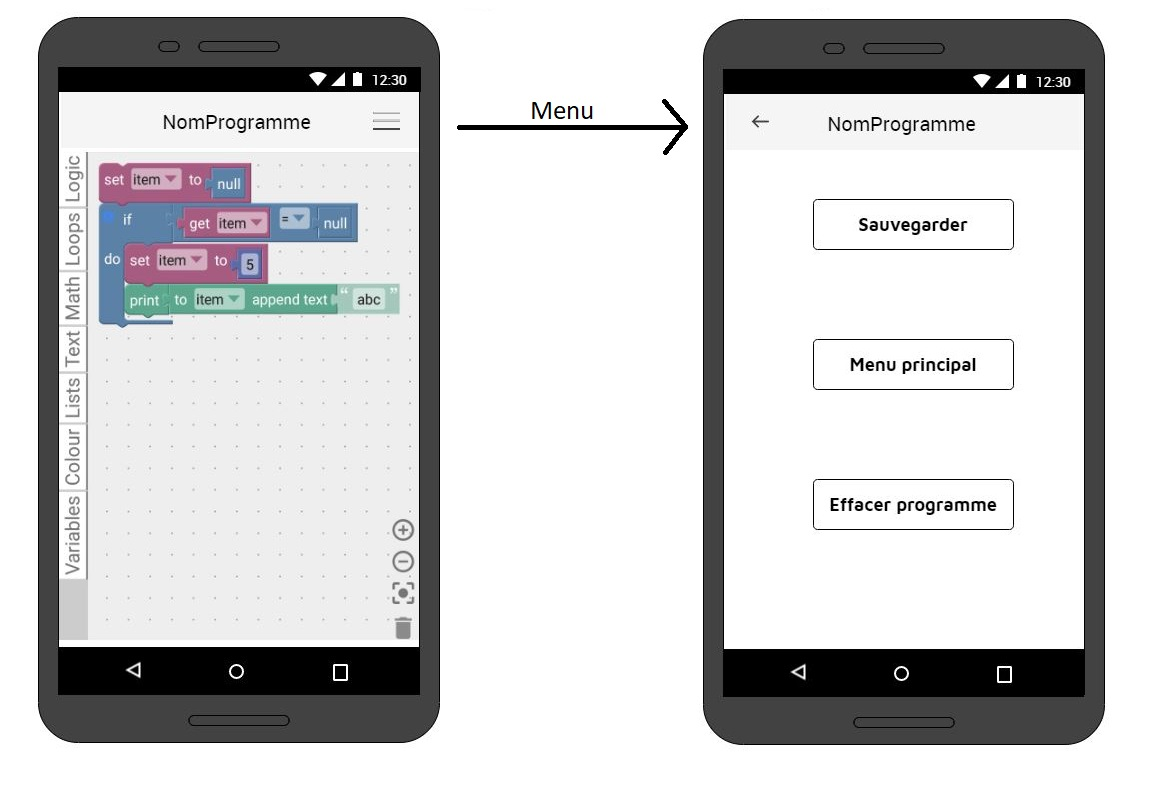
\includegraphics[scale=0.6]{./images/maquette2.jpg}~\\[1.5cm]
\caption{Maquette 2ème partie}
\label{figMaquette}
\end{addmargin}
\end{figure}



\chapter*{Architecture}

\begin{figure}[!h]
\begin{addmargin}[-4em]{1em}
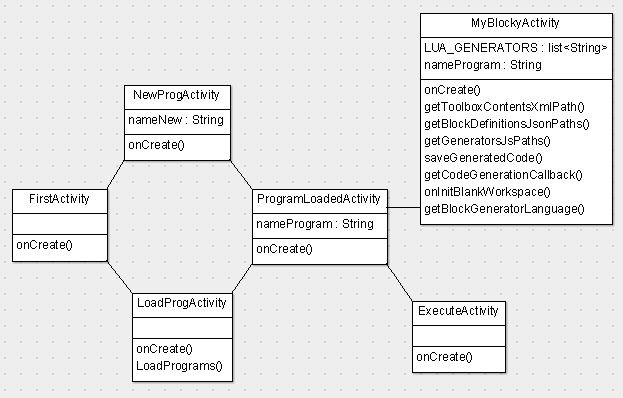
\includegraphics[scale=1.05]{./images/uml.jpg}~\\[1.5cm]
\caption{Architecture de l'application}
\end{addmargin}
\end{figure}

\newpage
\chapter*{Fonctionnement du système}

\section*{Exemples de fonctionnement}

Il est possible de créer deux types de programmes avec l'application, l'un concernant les blocs [pcDuino] qui seront traduits en Lua, et l'autre concernant les blocs [romeo] qui seront traduits en langage arduino.
Voici donc deux exemples de programmes Blockly pour chacune des cartes du robot :

\bigskip

Le premier programme concerne le pcDuino. Chaque programme doit être encadré par les blocs d'initialisation et de fermeture, afin que le code généré soit bien structuré. On voit ensuite 3 blocs identiques, qui mettent le sens des pins 1, 2 et 3 à 1. Ces 3 blocs permettent de dire au pcDuino que les pins concernés seront en mode écriture (contrairement au mode lecture, qui peut être utilisé avec des capteurs par exemple). On rentre ensuite dans une boucle qui sera exécutée 3 fois. Dans cette boucle, on allume un par un les pins 1, 2 et 3, qui correspondent dans cet exemple à une LED RGB, ou chaque couleur correspond à un pin. On en allume donc un par seconde, puis on les éteins tous grâce à un bloc qui regroupe les pins de la LED. Et enfin on ferme le programme.

\begin{figure}[!h]
\begin{addmargin}[-5.5em]{1em}
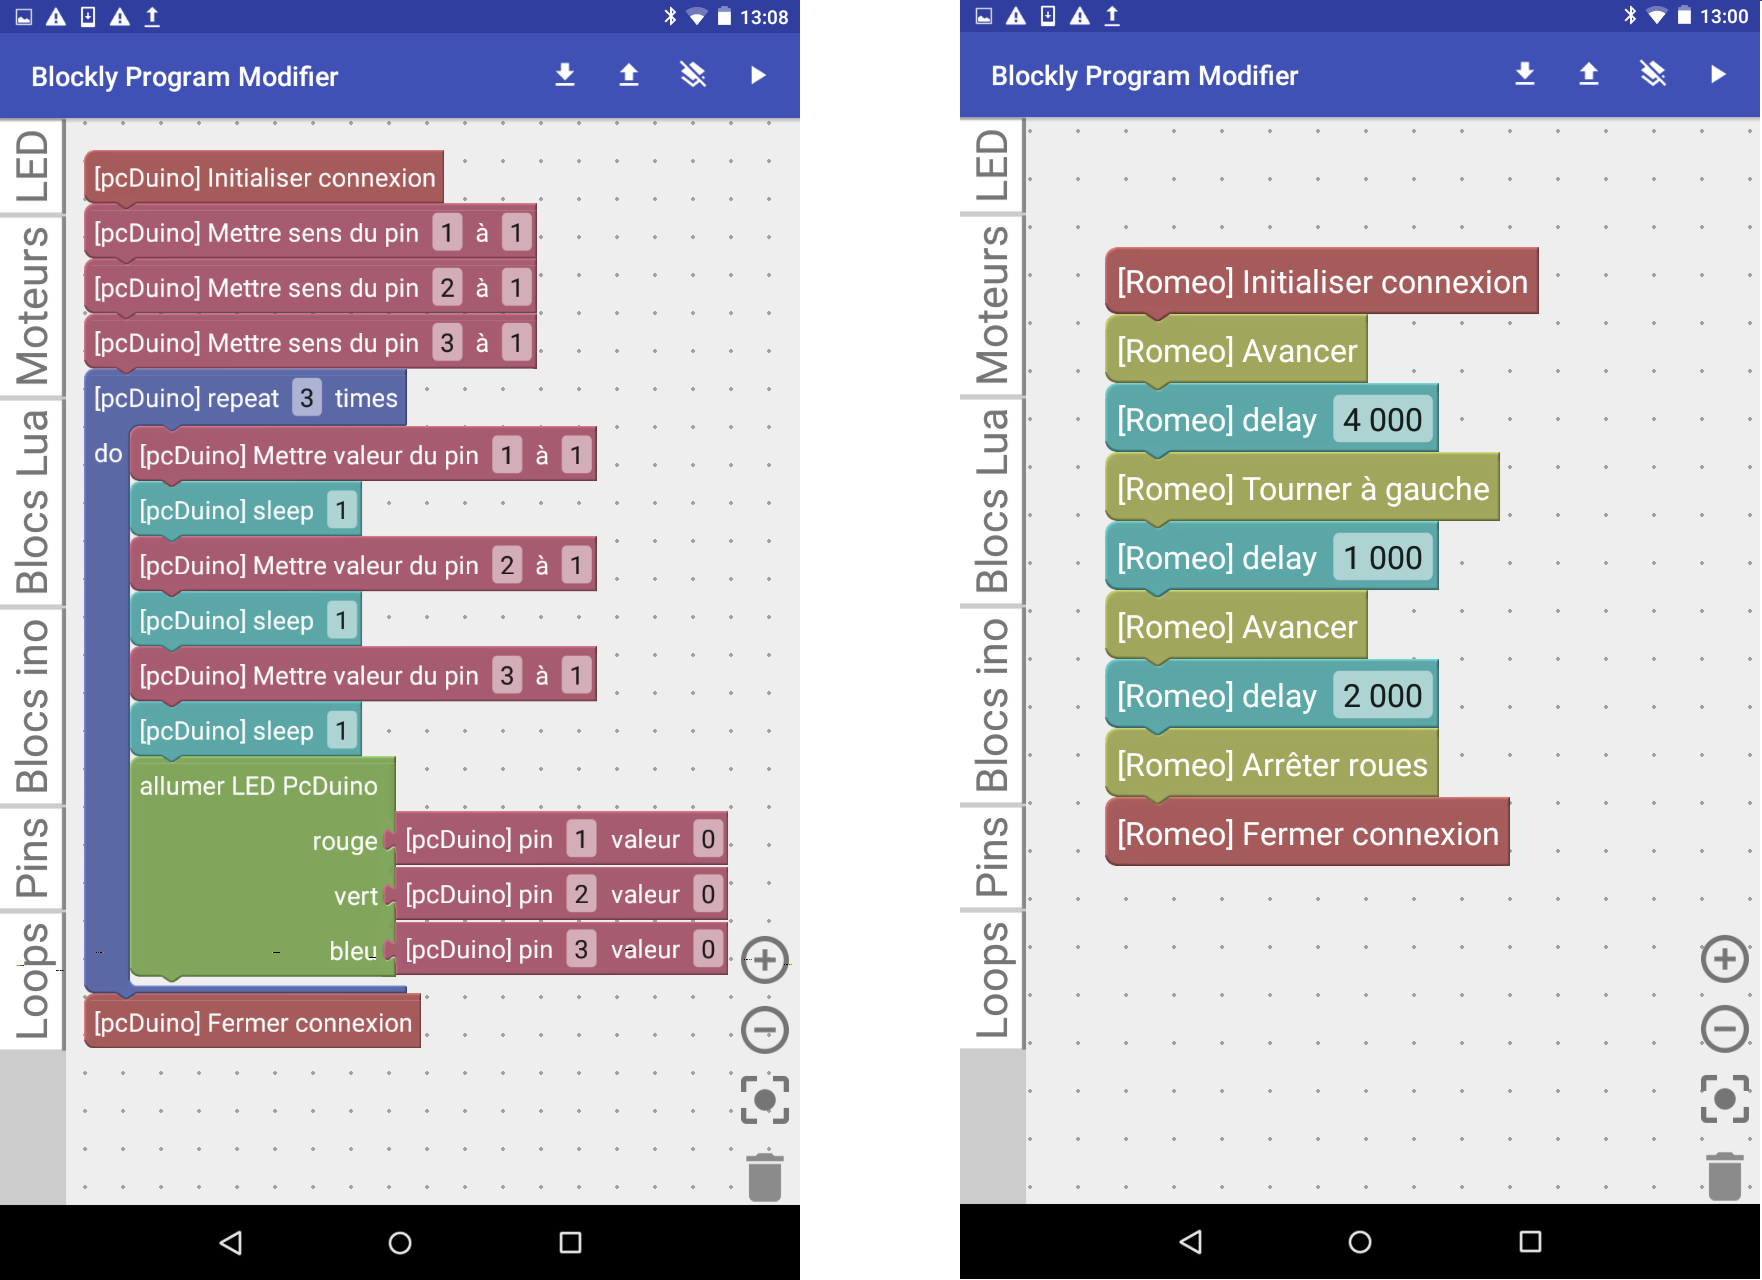
\includegraphics[scale=0.4]{./images/exemplePcDuino.png}~\\[1.5cm]
\caption{Exemples de programme pour le pcDuino et la Romeo}
\end{addmargin}
\end{figure}

\bigskip

Le second exemple concerne la Romeo, et plus précisément ses moteurs. Comme pour l'exemple précédent, il faut démarrer le programme avec un bloc d'initialisation. L'exécution du langage arduino sur la Romeo se faisant en boucle automatiquement, il n'y a pas besoin de mettre de boucle, à moins de souhaiter avoir une petite séquence du programme répétée plusieurs fois à l'intérieur même de la boucle principale. Dans ce code, on demande au robot d'avancer pendant 4 secondes, puis de tourner à gauche une seconde, et d'avancer à nouveau 2 secondes avant de s'arrêter. On termine encore une fois le programme avec un bloc de fermeture.

Ensuite quelque soit le type de programme en appuyant sur exécuter, le fichier généré sera envoyé par bluetooth au robot qui va l'exécuter.

\section*{Tests de validation}

Tous les tests de validation de l'application, comme du robot ont été faits à la main, car il n'est pas possible de faire de fonctions JUnit sur l'application du fait que la génération comme l'envoi du code nécessites une intervention humaine.

Nous avons donc fait des tests à 3 niveaux, ceux concernant l'application, ceux concernant le robot, et enfin ceux qui concernent la communication entre les deux appareils.

\paragraph*{Les tests sur l'application\\}

La fonction principale de l'application, et donc celle que nous avons testé est la génération du code à partir des blocs. Pour cela nous avons affiché le code généré dans la console, et testé la génération pour chaque bloc de la toolbox. Nous avons également testé le bon enregistrement du fichier en vérifiant son emplacement et son contenu.

\paragraph*{Les tests sur le robot\\}

Afin d'avancer étape par étape, avant de tester le fonctionnement global du système, nous avons testé la compilation et l'exécution du code pouvant être généré par les blocs en Lua et en Arduino. Pour cela nous avons écrit plusieurs programmes dans chaque langage afin de tester toutes les fonctionnalités possibles et de vérifier leur bon fonctionnement.
Nous avons également testé la partie du script qui compile et exécute les programmes indépendamment afin de s'assurer de sa bonne fonctionnalité.

\paragraph*{Les tests de communication\\}

La communication a été testée en 3 parties. La première a été d'envoyer des fichiers en bluetooth à d'autres appareils depuis l'application et de vérifier la réception et l'intégrité des données à l'arrivée. La seconde partie a été de lancer le script du pcDuino qui permet de recevoir des fichiers via bluetooth, et d'envoyer des fichiers de code depuis d'autres appareils pour vérifier qu'il recevait bien les fichiers et les exécutait immédiatement. Enfin nous avons fait des tests en conditions réels, c'est à dire en envoyant les fichiers générés par l'application grâce au bouton 'Exécuter', et en vérifiant que le robot effectuait bien la séquence d'instructions que nous avions écrit.

\chapter*{Partie technique}

\section*{Description technique}

\begin{description}
\item [Le pcDuino :] Le système d'exploitation du PcDuino est un Armbian basé sur la version 16 d'Ubuntu. Nous lui avons ajouté une clef Bluetooth ainsi que les commandes nécessaires à la réception des fichier envoyés par la tablette. De nombreux paquets ont été installés,notamment pour permettre la compilation et l'exécution de Lua, le téléversage vers la Romeo en lignes de commandes et l'utilisation du Bluetooth. 
Peu de code est stocké sur le pcDuino, seuls le script shell qui permet de recevoir des fichier via le bluetooth et de les compiler puis de les exécuter,ainsi que la librairie Lua sont nécessaires sur cette carte. Le reste de la configuration à été faite en ligne de commandes, ou dans des fichiers paramètres et n'a plus besoin d'être modifiée.
Le mot de passe de tous les utilisateurs du pcDuino (même root) est "ubuntu1234".
Pour modifier les valeurs des pins afin d'allumer ou éteindre les appareils branchés, il faut écrire dans des fichiers GPIO (Global Purpose Input Output)\cite{ref26} situés dans le système, et leur donner une valeur 1 pour les allumer, ou 0 pour les éteindre.

\item [L'application Android :] L'application android tourne sur notre tablette avec le sdk 22. 
Tous les fichiers contenant la description des blocs blockly, leur code, et la toolbox qui va avec se trouvent dans le dossier /assets/lua/ de l'application. Lors du lancement de l'application ils sont interprétés et affichés dans la page d'édition de programme. Une bibliothèque intégrés d'android permet à l'application de transmettre des fichiers par bluetooth au pcDuino.
Un générateur intégré à la bibliothèque blockly, ainsi que le code des blocks que nous avons créé, permettent de traduire le programme fait de blocs en un fichier de code Lua ou Arduino.

\item [Blockly :] Tous les blocks présents dans l'application ont été créés par notre groupe grâce à un outil Blockly en ligne prévu à cet effet, qui s'appelle "Blockly Developper Tools"\cite{ref25}. Cela nous a permis de choisir la forme du bloc, sa couleur, ses attributs, ses paramètres, les autres blocs qu'il accepte, etc. Ce même outil a permis de créer la toolbox personnalisée, dans laquelle on a regroupé les blocs par catégories. Enfin, le code correspondant a été écrit à la main, après que les fichiers aient été exportés. Tous ces fichiers sont ensuite passés à l'application android pour qu'elle les interprète.

\item [La Romeo :] La carte ne fait que recevoir et exécuter les programmes arduino qui sont téléversés depuis le pcDuino. Les moteurs contrôlant les roues du robot sont déjà branchées sur des pins spécifiques de la Romeo, et les autres pins sont libres afin d'y brancher n'importe quel appareil.

\end{description}

\section*{Limites du projet}



Lors de ce projet nous avons rencontré un certain nombre de problèmes qui ont freiné notre avancée, ou à cause desquels nous avons dû revoir certains objectifs :
\begin{itemize}
	\item Peut de temps après le choix de notre sujet nous avons dû changer d'enseignant, ce qui a entrainé un ralentissement dans notre rythme le temps que le nouveau responsable de notre groupe prenne connaissance du sujet.
	\item Nous avons aussi rencontré des problèmes matériels comme l'incapacité de pouvoir recharger les batteries des moteurs suite à l'absence d'une pièce. A l'heure actuelle, nous n'avons toujours pas de moyens de recharger les moteurs, mais nous avons réussi à obtenir une batterie de secours dans les derniers jours du projet, ce qui nous a laissé peu de temps pour tester nos blocs concernant les moteurs des roues. 
	\item Le pcduino étant relativement ancien les OS ne sont plus compatibles avec lui, nous en avions installé un qui était compatible avec les GPIO mais qui nous a empêché d'établir des connexions Wi-fi et bluetooth, car les paquets nécessaires n'étaient pas installés et ne pouvaient pas l'être. Nous avons donc dû chercher un OS plus récent, mais moins compatible avec le pcDuino. Nous avons finalement trouvé une version d'Armbian basée sur Ubuntu 16, qui supporte le bluetooth. En revanche cet OS a compliqué l'accès aux GPIO du pcDuino, et nous avons donc dû refaire notre librairie Lua.
	\item La dernière difficulté que nous avons rencontré est une incompatibilité entre le sujet et le matériel qui nous a été fourni, car le contrôle de la Romeo devait se faire en Lua mais la carte ne l'accepte pas, elle ne peut être contrôlée que par du langage Arduino. Nous avons donc dû dupliquer tous nos blocs afin de les traduire également en langage Arduino, pour pouvoir ensuite les exécuter sur la Romeo.	
\end{itemize}

\section*{Justification des algorithmes}

\section*{Analyse en complexité}

\section*{Extensions possibles}

\begin{itemize}

\item \textbf{Sauvegarde / chargement}

La sauvegarde / chargement faisait initialement partie des besoins fonctionnels de l'application. Par manque de temps cette fonctionnalité de basse priorité n'a pas été implémentée. Cette fonctionnalité permettrait la sauvegarde sur la tablette des programmes créés par l'utilisateur, ainsi que leur chargement. Il pourrait ainsi améliorer ou adapter ses programmes si le robot venait à évoluer.

Pour implémenter cette amélioration, il faudrait permettre à l'utilisateur de sauvegarder l'état actuel d'un programme. Cette sauvegarde se fera dans un fichier spécifique contenant les programmes sauvegardés ainsi que diverses informations (titre de la fonctionnalité, date de création …). À chaque démarrage de l'application, ce fichier sera chargé et les titres de programmes seront stocké dans une liste visible par l'utilisateur. Celui-ci pourra alors choisir d'afficher les détails d'un programme et de modifier son contenu.

\bigskip
\item \textbf{Refonte des blocs}

Actuellement, les blocs permettant d'utiliser une fonctionnalité du PcDuido sont marqués du label [pcDuino] et ceux permettant d'utiliser une fonctionnalité du Romeo sont marqués du label [romeo].
Le code généré à partir de blocs contenant le label [pcDuino] est en langage Lua contrairement à celui généré à partir des blocs contenant le label [romeo] qui est en langage Arduino.

Cette distinction a été faite à cause de l'impossibilité d'exécuter du Lua sur la Romeo. Lors de la création de notre application, nous pensions l'exécution de code Lua sur la Romeo possible. En conséquence, nous avons défini la forme de nos blocs de telle manière qu'il est possible d'imbriquer des blocs correspondants à du code Lua avec des blocs correspondant à du code Arduino. Bien évidemment, ces blocs ne doivent pas être utilisés ensemble dans un même programme pour ne pas provoquer un échec de la compilation.

Une amélioration possible de notre application sera de repenser totalement la forme de nos blocs, afin que les blocs ayant le label [pcDuino] ne soient plus imbricables avec ceux possédant le label [romeo].

\bigskip
\item \textbf{Outil de création et d'ajout de blocs pour un développeur}

Actuellement, les blocs de la toolbox sont ceux que nous avons définis en correspondance avec les divers capteurs et actionneurs du robot. Si le robot évolue, il serait intéressant de pouvoir supprimer ou ajouter de nouveaux blocs. 

Pour ajouter un nouveau bloc, il faut trois éléments :
un fichier block.json décrivant le blocs (couleur, forme, ce qu'il reçoit, etc)
un fichier block.js contenant le code généré par le bloc
un fichier toolbox.xml contenant les catégories auxquelles le bloc appartient

Un outil pourrait être développé pour faciliter l'ajout d'un nouveau bloc à l'application. Cet outil demanderait les emplacements des fichiers .json et .js sur la tablette et se chargerait d'ajouter leur contenu aux fichiers déjà existant contenant le reste des blocs. Par la suite, un menu déroulant permettrait de choisir les catégories auxquelles le nouveau bloc appartient parmi celles déjà existantes. Il serait aussi possible de créer de nouvelles catégories. Cet outil permettrait également la suppression de blocs déjà existants.

\bigskip
\item \textbf{Amélioration de l'application côté robot}

Actuellement, le robot se contente d'exécuter un script après le démarrage. Ce script contient une boucle infinie qui va vérifier la présence de code Lua ou Arduino envoyé depuis la tablette et l'exécuter si ce code existe.

On pourrait imaginer remplacer ce script par un programme, écrit dans un langage quelconque, qui en plus de proposer l'exécution de code envoyé depuis la tablette proposerait des fonctionnalités supplémentaires. Une fonctionnalité pourrait être l'envoi par bluetooth d'une liste contenant les équipements installés et actifs sur le robot. Cette liste permettrait à l'application android de modifier la liste des blocs disponibles dans la toolbox. Par exemple, si les capteurs infrarouges venaient à être retirés du robot ou à tomber en panne, les blocs utilisant ces capteurs ne seraient plus affichés dans la liste des blocs disponibles.

\end{itemize}

\chapter*{Annexes}

\section*{Manuel d'utilisation}



\bibliographystyle{unsrt}
\bibliography{biblio}

\end{document}
